
%%%%%%%%%%%%%%%%%%%%%%% file typeinst.tex %%%%%%%%%%%%%%%%%%%%%%%%%
%
% This is the LaTeX source for the instructions to authors using
% the LaTeX document class 'llncs.cls' for contributions to
% the Lecture Notes in Computer Sciences series.
% http://www.springer.com/lncs       Springer Heidelberg 2006/05/04
%
% It may be used as a template for your own input - copy it
% to a new file with a new name and use it as the basis
% for your article.
%
% NB: the document class 'llncs' has its own and detailed documentation, see
% ftp://ftp.springer.de/data/pubftp/pub/tex/latex/llncs/latex2e/llncsdoc.pdf
%
%%%%%%%%%%%%%%%%%%%%%%%%%%%%%%%%%%%%%%%%%%%%%%%%%%%%%%%%%%%%%%%%%%%


\documentclass[runningheads,a4paper]{llncs}

\usepackage[utf8]{inputenc}
\usepackage[T1]{fontenc}
\usepackage{caption}
\usepackage{subcaption}
\usepackage{amssymb}
\setcounter{tocdepth}{3}
\usepackage{graphicx}
\graphicspath{ {./images/} }
\usepackage{hyperref}
\usepackage{url}
\usepackage{listings, chngcntr}
\usepackage{color}
\definecolor{lightgray}{rgb}{.9,.9,.9}
\definecolor{darkgray}{rgb}{.4,.4,.4}
\definecolor{purple}{rgb}{0.65, 0.12, 0.82}

\lstdefinelanguage{JavaScript}{
  keywords={typeof, new, true, false, catch, function, return, null, catch, switch, var, if, in, while, do, else, case, break},
  keywordstyle=\color{blue}\bfseries,
  ndkeywords={class, export, boolean, throw, implements, import, this},
  ndkeywordstyle=\color{darkgray}\bfseries,
  identifierstyle=\color{black},
  sensitive=false,
  comment=[l]{//},
  morecomment=[s]{/*}{*/},
  commentstyle=\color{purple}\ttfamily,
  stringstyle=\color{red}\ttfamily,
  morestring=[b]',
  morestring=[b]"
}

\lstset{
   language=JavaScript,
   extendedchars=true,
   basicstyle=\footnotesize\ttfamily,
   showstringspaces=false,
   showspaces=false,
   numbers=left,
   numberstyle=\footnotesize,
   numbersep=9pt,
   tabsize=2,
   breaklines=true,
   showtabs=false,
   captionpos=b
}

\newcommand{\keywords}[1]{\par\addvspace\baselineskip

\noindent\keywordname\enspace\ignorespaces#1}

\begin{document}

\counterwithin{lstlisting}{section}

\mainmatter  % start of an individual contribution

% first the title is needed
\title{TypeDevil: Dynamic Type Inconsistency Analysis for JavaScript\\-\\Seminar Report}

% a short form should be given in case it is too long for the running head
\titlerunning{TypeDevil - Seminar Report}

% the name(s) of the author(s) follow(s) next
\author{Nico Fechtner}
%
\authorrunning{Seminar Report: TypeDevil}
% (feature abused for this document to repeat the title also on left hand pages)

% the affiliations are given next; don't give your e-mail address
% unless you accept that it will be published
\institute{Technical University of Munich\\
Department of Informatics\\
Chair for IT Security\\
Boltzmannstraße 3, 85748 Garching, Germany\\
\href{mailto:nico.fechtner@tum.de}{nico.fechtner@tum.de}
}

%
% NB: a more complex sample for affiliations and the mapping to the
% corresponding authors can be found in the file "llncs.dem"
% (search for the string "\mainmatter" where a contribution starts).
% "llncs.dem" accompanies the document class "llncs.cls".
%

% ???
\toctitle{}
\tocauthor{}
\maketitle
% \newpage

\tableofcontents
\newpage

\begin{abstract}
JavaScripts dynamic and weak type system which makes it possible to write type inconsistent and therefore buggy code. 
TypeDevil addresses this issue with a mostly dynamic type inconsistency analysis which is able to effectively warn developers about critical type related bugs.
An alternative solution heavily used in real world projects are additional static type system like e.g. TypeScript.
A comparing evaluation shows that both approaches perform quite similar in finding type inconsistencies with TypeScript being just slightly better.
%\keywords{Dynamic Type Inconsistency Analysis for JavaScript, TypeDevil, Static Type Systems for JavaScript, TypeScript}
\end{abstract}

\newpage

\section{Introduction}

This report is part of the seminar "Common Security Flaws in JavaScript based Applications", which was organized by Paul Muntean from the Chair of IT Security at the Faculty of Informatics of the Technical University of Munich.
The seminar took place in the summer semester 2018 and dealt with multiple scientific papers related to JavaScript Security. \\
I personally took a deeper look at the paper "TypeDevil: Dynamic Type Inconsistency Analysis for JavaScript", published in 2014 by Michael Pradel, Parker Schuh and Koushik Sen.
In this report I would like to explain the general problem the paper tries to address, introduce TypeDevil as a possible solution and compare TypeDevil to an alternative approach, namely additional static type systems. 

\section{Inconsistent Types as the Root Cause of Many Bugs}
First of all, I would like to introduce the general problem, TypeDevil addresses. \\
JavaScript as a programing language features two striking characteristics we will focus on. 
On the one hand, JavaScript is dynamically typed. 
This basically means, that we do not provide any static type annotations to our source code, like you would do in statically typed languages, such as e.g. Java, and that types - for example of local variables - can change during runtime.
On the other hand, JavaScript is also weakly typed and thereby very permissive. In order to prevent runtime exceptions, JavaScript performs a lot of automatic type conversions, also known as implicit coercions.
Consider the code example in listing \ref{listingPets}. 
One could expect the script to print \lstinline[columns=fixed]{"Cat Dog Rabbit "} to the console.
The actual output however is \lstinline[columns=fixed]{"undefinedCat Dog Rabbit "}. 
In the first iteration of the for-loop, we try to concatenate a string to the value of \lstinline[columns=fixed]{outputString}, which is undefined. 
JavaScript now performs a implicit coercion and converts the value \lstinline[columns=fixed]{undefined} to the string \lstinline[columns=fixed]{"undefined"} which leads to the unexpected output.
\\ \\
\lstset{language=javascript}
\begin{minipage}{\linewidth}
\begin{lstlisting}[frame=single, caption=Implicit Coercions, label={listingPets}] 
var pets = ["Cat", "Dog", "Rabbit"];

var outputString;

for (var i in pets) {
    outputString += pets[i] + " ";
}

console.log(outputString);
\end{lstlisting}
\end{minipage}

As we saw, dynamic languages do not require programmers to annotate their programs with type information or to follow any strict typing discipline. 
This freedom allows developers to write concise code in short time. 
However, most code does follow implicit type rules, e.g. only a single type per variable or object property or fixed function signatures.
The authors of TypeDevil further state that many bugs are actually violations of these rules.
So the freedom offered by dynamic languages often comes at the cost of hidden bugs and since the language does not enforce any typing discipline, no compile-time warnings are reported if a program uses and combines types inconsistently.
Although the code example does not seem that harmful, when you consider business sensitive services like authentication or payment libraries, of course even a little type error could do some real damage. \\
TypeDevil wants to address this problem by gathering type observations during run-time, summarizing them into a type graph and finally reporting a set of aggressively filtered type inconsistency warnings.
The challenges are on the one hand the absence of static type information and on the other hand the fact that a lot of JavaScript code is polymorphic on purpose and the tool shouldn't report false positives when encountering intended polymorphic constructs.

\section{Static and Dynamic Analyses} \label{staticDynamicAnalysis}

For better understanding of the following I would like to clarify the difference between static and dynamic analyses first.\\
The key differentiation point is that within a static analysis you do not have any runtime information, since the analysis runs ahead of time and the only input to the analysis is the source code itself.
Therefore it is usually quite hard to predict the exact program behavior.
It turns out, that it is even harder to get comprehensive and precise results for dynamic languages like JavaScript, because of constructs like the \lstinline[columns=fixed]{eval()} function, which interprets the string passed to it at runtime as normal JavaScript code. 
However the good part about static analysis is that it usually covers all code paths and runs quite fast.
Typical examples for static analyses in the context of JavaScript are linters, like ESLint, JSLint or Prettier, which can "detect common programming errors and ensure that certain best practices are followed". \\
Dynamic analyses are typically characterized through the fact that they do have access to runtime information.
Often, instrumentation code gets added to the original source code to keep track of certain characteristics of the program the analysis cares about.
After that, this instrumented version of the source code gets executed, the analysis gathers runtime information, e.g. user input, and the results of the analysis get computed.
With this approach you can catch certain errors, static analysis wouldn't be able to find.
For example, consider again the \lstinline[columns=fixed]{eval()} function.
With a dynamic analysis you can actually track the code which gets interpreted on the fly.
However, the biggest downside of a purely dynamic analysis is, that it can not cover all code paths most of the time.
TypeDevil uses a mostly dynamic approach to gather type observations at runtime.

\section{TypeDevils Approach}

This section will introduce you to the mechanisms TypeDevil uses to effectively identify and report inconsistent types.
In general, there are three main phases, TypeDevil goes through: 
First, instrumentation code gets inserted to the original source code to gather type observations at every relevant point in the program execution.
Out of this potentially huge set of type observations, TypeDevil constructs a type graph, which makes it possible to merge types which are structurally equivalent relatively easily.
On the basis of the condensed type graph, TypeDevil identifies inconsistent types and applies a set of merging and pruning techniques to drastically reduce the number of reported warnings.

\subsection{Running Example}
Consider listing \ref{listingRunningExample}, which shows the running example I will use to introduce you to the various steps of TypeDevils pipeline.
Note that this is also the example, the authors of TypeDevil used throughout their paper.
As you can see, there is a simple function \lstinline[columns=fixed]{addWrapped} which takes two arguments and returns the addition of the \lstinline[columns=fixed]{v} properties of both arguments if you pass two parameters and returns just the \lstinline[columns=fixed]{v} property of the first argument if only one is passed at the function call.
Then there is a simple constructor function \lstinline[columns=fixed]{Wrapper} which just creates an object with only one property \lstinline[columns=fixed]{v}.
And lastly \lstinline[columns=fixed]{addWrapped} gets called three times with different parameters.
Of course it sticks out that the \lstinline[columns=fixed]{v} property of the object we pass to \lstinline[columns=fixed]{addWrapped} when calling it the third time is a string and not a number.
This seems to be a type inconsistency and as we will see, TypeDevil will effectively warn us about this problem.
\\ \\
\lstset{language=javascript}
\begin{minipage}{\linewidth}
\begin{lstlisting}[frame=single, caption=Running Example, label=listingRunningExample]
function addWrapped(x, y) {
    if (y) {
        return x.v + y.v;
    } else {
        return x.v;
    }
}

function Wrapper(v) {
    this.v = v;
}

addWrapped({v:23});
addWrapped({v:20}, new Wrapper(3));
addWrapped({v:"18"}, new Wrapper(5));
\end{lstlisting}
\end{minipage}


\subsection{Gathering Type Observations}

The first phase of TypeDevil is to gather type observations at runtime.
To achieve this, TypeDevil instruments the original source code in two ways.
On the one hand, a shadow value gets added to each object and function, containing a unique identifier, which makes it easy to access the objects of functions type name whenever they are referred to. 
On the other hand, TypeDevil saves type observations at every relevant code location to a global set.
In the sense of TypeDevil, a type is either a primitive type (boolean, number, string, undefined, null) or a so called record type, which basically maps a named property to a set of types.
For record types, TypeDevil differentiates between object types, array types, function types and (function) frame types.
A type observation is therefore a triple consisting of a basetype, a property and an observed type.
In the following, we will look at each instrumentation, TypeDevil adds to the original source code of our running example.

\subsubsection{Object Literals}
Consider \lstinline[columns=fixed]{addWrapped} gets called for the first time.
With the object literal \lstinline[columns=fixed]!{v:23}! we create a new object to pass it to the function.
First, we append a shadow value holding a unique identifier to the newly created object. A possible unique identifier could just be the string \lstinline[columns=fixed]{"object"} concatenated with a unique number, e.g. \lstinline[columns=fixed]{"object1"}.
After that, we add a type observation for each property of the object.
In our example we would add the type observation \lstinline[columns=fixed]{(object1, v, number)}, since \lstinline[columns=fixed]{"object1"} is the basetype, \lstinline[columns=fixed]{v} is the name of the property and \lstinline[columns=fixed]{23} is a numeric value.

\subsubsection{Property Access}
TypeDevil also gathers type observations on each property access.
In our example, when we call \lstinline[columns=fixed]{addWrapped} for the first time, we do not provide a second argument, so we will definitely end up in the else branch on line 5. 
There we access the property \lstinline[columns=fixed]{v} of the object we passed to the function.
So we add the type observation \lstinline[columns=fixed]{(object1, v, number)}.
As you can see, this is exactly the same type observation we already stored at the creation of the object which seems quite redundant at the first glance. 
Nevertheless we have to add a type observation for each property access, since code which we do not instrument like third party libraries or code which we just cannot instrument, namely native code, could potentially change the types of properties.

\subsubsection{Function Literals}
Just as we saw on the example of objects, TypeDevil also appends shadow values containing unique identifiers to all function literals.
In our example, it would append the unique identifier \lstinline[columns=fixed]{"function addWrapped"}, to the function starting at line 1.

\subsubsection{Function Calls}
For each function call, TypeDevil adds two type observations.
The first one refers to the receiver of the function and the second one refers to the return type.
Consider again the first call of \lstinline[columns=fixed]{addWrapped}.
TypeDevil adds the type observation \lstinline[columns=fixed]{(function addWrapped, this, window)}, since \lstinline[columns=fixed]{addWrapped} gets called without an explicit receiver in which case the global object - e.g. \lstinline[columns=fixed]{window} - becomes the receiver
and \lstinline[columns=fixed]{(function addWrapped, return, number)}, since the function returns a numeric value (\lstinline[columns=fixed]{23}).

\subsubsection{Variable Access}
We already saw how TypeDevil gathers type observations for each property access.
Analogical to that TypeDevil deals with local variable accesses.
It is important to note, that similar to the internal implementation of JavaScript itself, TypeDevil treats function arguments as local variables.
Like in the previous examples, consider the first call of \lstinline[columns=fixed]{addWrapped}.
TypeDevil adds the type observation \lstinline[columns=fixed]{(frame addWrapped, y, undefined)} when the value of \lstinline[columns=fixed]{y} gets accessed, which happens to be \lstinline[columns=fixed]{undefined}.

\subsection{Executing the Program}
After instrumenting the original source code, TypeDevil executes the program and dynamically gathers type observation for each construct mentioned above.
The authors of TypeDevil implemented two versions of the analysis. 
You can either run it on top of node or you can use a custom version of Firefox where they modified Spidermonkey, the JavaScript engine of Firefox, to instrument the JavaScript programs before they get executed.
After the instrumented execution TypeDevil holds a huge set of type observations for further processing.

\subsection{Building the Type Graph and Identifying Inconsistent Types}

\begin{figure}
    \centering
    \begin{subfigure}{.5\textwidth}
      \centering
      \includegraphics[width=.4\linewidth]{image1}
      \caption{A subfigure}
      \label{fig:sub1}
    \end{subfigure}%
    \begin{subfigure}{.5\textwidth}
      \centering
      \includegraphics[width=.4\linewidth]{image1}
      \caption{A subfigure}
      \label{fig:sub2}
    \end{subfigure}
    \caption{A figure with two subfigures}
    \label{fig:test}
    \end{figure}
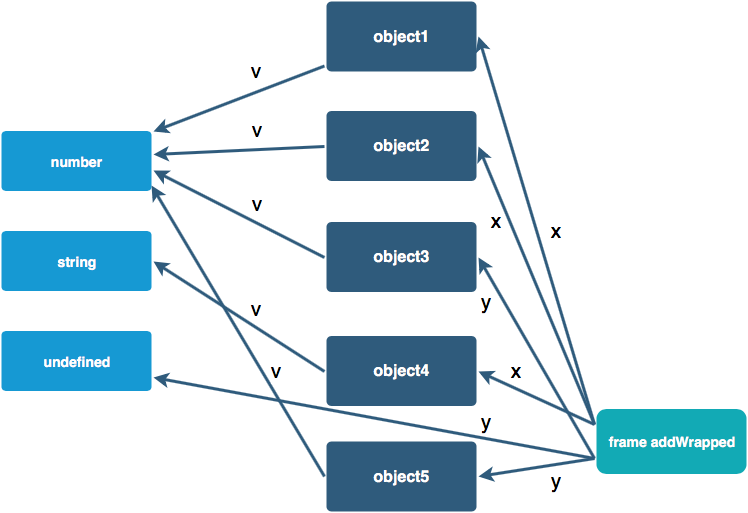
\includegraphics[width=\textwidth]{UncondensedTG}
\caption{Uncondensed Type Graph}
\end{figure}

\begin{figure}[h]
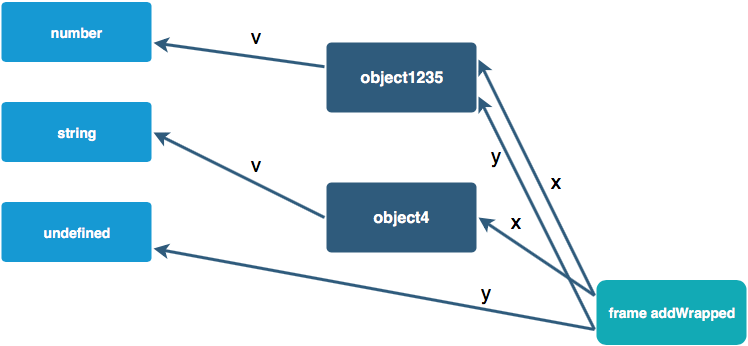
\includegraphics[width=\textwidth]{CondensedTG}
\caption{Condensed Type Graph}
\end{figure}


\subsection{Merging and Pruning of Warnings}


\section{Related Research}

First of all, there is a lot of related research on static type analysis.
While the first publications in this field restricted JavaScript to a subset which was suitable for static analysis, \cite{DBLP:conf/sas/JensenMT09} showed that it is also possible to perform an effective static type inconsistency analysis while allowing the whole JavaScript language.
Of course also for type analyses the typical advantages and disadvantages of static analysis explained in \ref{staticDynamicAnalysis} hold true.
In the field of dynamic type analysis for JavaScript, TypeDevil is still the state of the art approach, according to \cite{DBLP:conf/icse/TanXCLYS17}. 
\cite{DBLP:conf/icse/TanXCLYS17} also implemented a combined type analysis which first analyzes programs statically and afterwards refines the results with a subsequent dynamic analysis which implements the basic ideas of TypeDevil.
Another research area which tries to solve the general problem of type inconsistencies for dynamic languages is the field of additional type checkers.
We will take a closer look at this approach in the following section.

\section{Static Type Systems as an Alternative to Dynamic Analysis}

Additional static type systems for JavaScript got a lot of attention over the last years, since major tech companies like Google, Facebook or Microsoft are developing them and provide production ready tools for developers.
They basically try to solve the same problem as TypeDevil.
They want to provide developers with warnings for type inconsistent code, but in contrast to dynamic analyses like TypeDevil you already get these warnings ahead of time.
Note that static type systems for dynamic languages also have a lot of additional advantages.
For example they enable a mature development experience with rich auto completion, advanced refactoring options and always up-to-date code documentation.
However, in the following we will just focus on type warnings.

\subsection{Approach of Additional Static Type Systems} \label{staticTypeSystems}
There are a lot of different additional static type systems - also known as static type checkers - for JavaScript.
The three most used ones are TypeScript (Microsoft), Flow (Facebook) and the Google Closure Compiler.
Basically they all work quite similar.
Most of them are a super set of JavaScript, which simply means that every valid JavaScript program is also already for example a TypeScript or a Flow program.
This makes the gradual adoption of an additional type system really easy.
The basic approach is to extend the core JavaScript language with additional type annotations, either in the form of inline types (TypeScript, Flow) or in the form of special comments (Google Closure).
Another characteristic of static type checkers is their mature type inference, which means that you do not have to provide special type annotations at any point in your program per se.
Instead, the tools try to infer most of the types for you. 
For example, when you declare and initialize a variable to a numeric value, the inferred type for that variable would be \lstinline[columns=fixed]{number}.
If you afterwards try to assign e.g. a string value to this variable, you would get a compiler warning without having to explicitly declare that this variable should only hold numeric values.


\subsection{Introduction to TypeScript}
To give you the necessary background for the upcoming comparison in \ref{comparison}, I would like to introduce you to TypeScript.
I choose TypeScript as an example for a static type checker, since it is by far the most used one according to \cite{StateOfJs}.
Furthermore, \cite{DBLP:conf/icse/GaoBB17} showed, that in terms of type inconsistencies, TypeScript and Flow report nearly the exact same warnings.
As stated in \cite{DBLP:conf/ecoop/BiermanAT14}, TypeScript is a syntactic superset of JavaScript, which provides additional syntax for declaring and expressing types, for annotating properties, variables, parameters and return values with types, and for asserting the type of an expression.
However, as explained in \ref{staticTypeSystems}, TypeScript also supports rich type inference.
For example, consider the example shown in Listing \ref{listingForEach}.
Without any modification of the source code, you would get the following warning, when compiling this script with the TypeScript compiler:
\lstinline[columns=fixed]{Operator '+=' cannot be applied to types 'number' and 'number | boolean'}.
So TypeScript notes, that the property \lstinline[columns=fixed]{a} of the objects which the program iterates over is sometimes a numeric and sometimes a boolean value and prevents you from writing type inconsistent code like this.

\medskip\medskip
\lstset{language=javascript}
\begin{minipage}{\linewidth}
\begin{lstlisting}[frame=single, caption=inconsistent\_foreach.js, label=listingForEach]
(function() {
    
    var a = [{a: 23}, {a: 42}, {a: false}];
    var sum = 0;
    a.forEach(function(x) {
        sum += x.a;
    });
    
})();
\end{lstlisting}
\end{minipage}



\section{Evaluation}

\subsection{Original Results for TypeDevil}

\subsection{Comparing TypeDevil and TypeScript} \label{comparison}

\subsubsection{Evaluation Setup}

\subsubsection{Results}


\subsection{Discussion}



\section{Conclusion and Future Work}


\bibliography{my}{}
\bibliographystyle{plain}
\end{document}
